\section{Literature Review}

\textbf{Realized volatility.} Summing squared intraday returns gives realized variance (RV), a
model-free estimate of the day's integrated variance \citep{andersen2003}. Five-minute sampling is
hard to beat across asset classes \citep{liu2015}, and simple models of RV forecast better than
GARCH models fitted to daily returns \citep{andersen2003}.

\textbf{HAR-RV.} \citet{corsi2009} regresses tomorrow's RV on its daily, weekly and monthly
averages. Four parameters reproduce the long memory of volatility, and the model is still the
standard benchmark. Estimating it in logs reduces the weight of a few extreme days on the
coefficients.

\textbf{EGARCH and hybrids.} EGARCH \citep{nelson1991} models log variance from daily returns and
allows bad news to raise volatility more than good news. \citet{kim2018} feed GARCH-family outputs
into an LSTM \citep{hochreiter1997} for the KOSPI 200 and report gains over both parts.

\textbf{Machine learning against HAR.} \citet{bucci2020} finds recurrent networks beat HAR models
for US equity RV. Large DJIA studies are more sceptical: \citet{rahimikia2020} find gains mainly in
calm periods, and \citet{christensen2023} find they depend on covariates and the evaluation window.
Pooling many stocks in one network helps \citep{zhang2024}. Almost all of this evidence is for
liquid US stocks; whether the gain depends on liquidity, and whether it holds in an emerging market,
is largely untested.

\textbf{Evaluation.} RV is itself an estimate, so the loss must rank forecasts correctly under a noisy
proxy; MSE and QLIKE do, and QLIKE is less sensitive to extreme days \citep{patton2011}. Forecasts are
compared with the Diebold--Mariano test \citep{diebold1995}, with Newey--West standard errors
\citep{neweywest1987}.

\section{Data}

\subsection{Source and cleaning}

The data are 5-minute bars (open, high, low, close, volume) for 100 current NIFTY~100 stocks on the
NSE, February 2015 to 9 April 2026 (18.8 million bars). The regular session runs 09:15--15:30 IST, so
a full day has 75 bars. Prices are mostly adjusted for corporate actions, but the files contain
pre-listing quotes, zero prices, special sessions and isolated bad prints. Table~\ref{tab:cleaning}
lists the rules; all are set in one configuration file.

\begin{table}[htbp]
\centering
\caption{Data cleaning rules and their effect}
\label{tab:cleaning}
\small
\begin{adjustbox}{max width=\textwidth}
\begin{tabular}{lcr}
\toprule
Rule & Action & Count \\
\midrule
Raw 5-minute bars, 100 stocks & -- & 18,798,744 \\
Regular session 09:15--15:30, from Nov 2015, after listing date & Keep & 17,660,206 \\
Zero-volume bars (stale quote, price set to missing) & Drop price & 41,063 \\
Isolated spikes ($>$5\% move undone by next bar) & Drop price & 24 \\
Days with fewer than 60 traded bars & Drop day & 1,455 \\
Days with RV $=0$ (stock frozen at price band) & Drop day & 188 \\
Overnight gaps $>35\%$ (split/bonus) in EGARCH returns & Set to 0 & 2 \\
Stock-days in the clean panel & -- & 234,226 \\
\bottomrule
\end{tabular}
\end{adjustbox}
\par\smallskip\parbox{0.95\textwidth}{\footnotesize\itshape Pre-listing rows removed for IRFC, SBILIFE, HDFCLIFE and MAZDOCK. RV never uses overnight returns.}
\end{table}


The most volatile stock-days left after cleaning are real events: the Adani sell-off of 1--3 February
2023 and the COVID-19 crash of March 2020 (Annex Table~\ref{tab:topdays}).

\subsection{Realized variance and returns}

Let $r_{i,t,j}$ be the $j$-th 5-minute log return of stock $i$ on day $t$, with the first return measured
from the day's first traded open. Realized variance is
\begin{equation}
RV_{i,t}=\sum_{j=1}^{M_{i,t}} r_{i,t,j}^{2}, \qquad M_{i,t}\le 75 .
\end{equation}
RV covers the trading session only; the overnight gap is excluded, which keeps unadjusted splits,
bonus issues and demergers out of the target. Annualized volatility is $\sqrt{252\,RV}$. Daily
close-to-close returns for EGARCH add the overnight return, set to zero on the two days where it
exceeded 35\% in absolute value (a corporate action, not a price move).

\subsection{Sample split and universe}

Each observation is assigned to a period by the date of the \emph{target} (day $t+1$): training
2016--2022, validation 2023--2024 (early stopping only), and test 1 January 2025 -- 9 April 2026,
which was not used for any choice. The universe is the 95 stocks with at least 250 training days;
five recent listings (Hyundai, Jio Financial, Tata Capital, TMCV, ENRIN) are excluded.

\subsection{Liquidity groups}

Liquidity is measured with the 5-minute Amihud ratio \citep{amihud2002},
\begin{equation}
ILLIQ_i=\frac{1}{N_i}\sum_{k}\frac{|r_{i,k}|}{\text{Rupee volume}_{i,k}},
\end{equation}
averaged over all traded 5-minute bars in the \emph{training} years only, so group membership uses
no information from the evaluation period. A low ILLIQ means trades move the price little. Stocks are
split into terciles: High (32 stocks), Medium (31) and Low liquidity (32). The ranking agrees with
traded value (Spearman $-0.91$): Reliance, SBI, Infosys and ICICI Bank are the most liquid; CG Power,
Solar Industries and Trent the least (Figure~\ref{fig:liq}).

\begin{figure}[htbp]
\centering
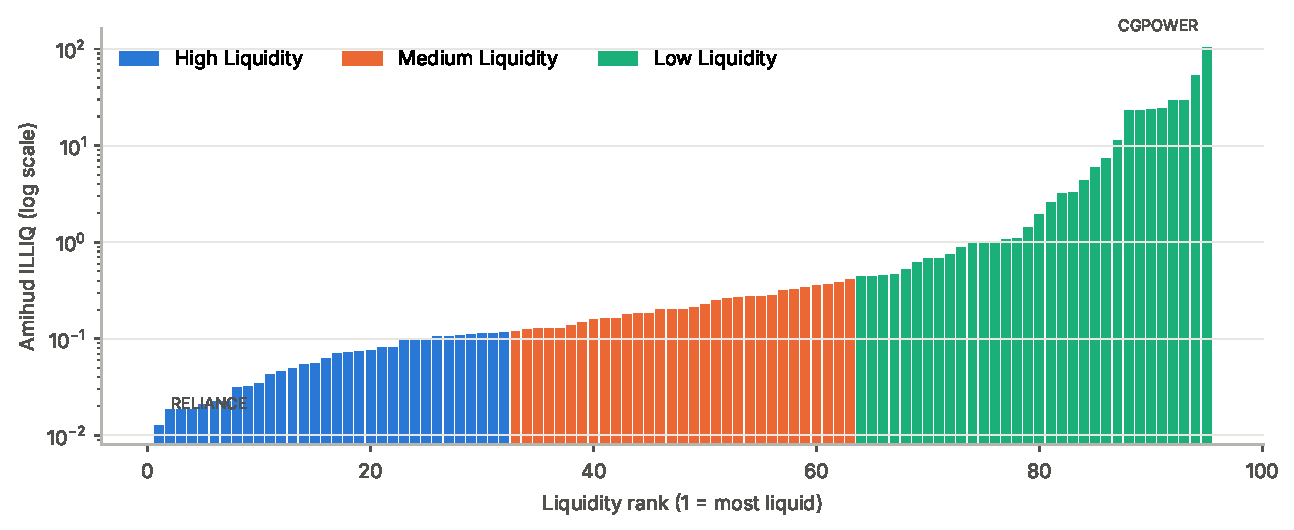
\includegraphics[width=\textwidth]{fig_liquidity_ranking.pdf}
\caption{Amihud illiquidity of the 95 stocks in the training years (log scale), coloured by tercile.}
\label{fig:liq}
\end{figure}

\begin{table}[htbp]
\centering
\caption{The three liquidity groups, 2016--2026}
\label{tab:desc}
\small
\begin{adjustbox}{max width=\textwidth}
\begin{tabular}{lrrrrrrr}
\toprule
Liquidity & Stocks & Stock-days & Turnover (Rs cr/day) & Mean vol (\%) & Median vol (\%) & 99th pct vol (\%) & AR(1) log RV \\
\midrule
High & 32 & 80,742 & 533 & 25.1 & 22.0 & 75.6 & 0.70 \\
Medium & 31 & 78,064 & 193 & 28.5 & 25.3 & 81.4 & 0.65 \\
Low & 32 & 73,900 & 142 & 33.1 & 28.4 & 103.8 & 0.65 \\
\bottomrule
\end{tabular}
\end{adjustbox}
\par\smallskip\parbox{0.95\textwidth}{\footnotesize\itshape Vol = annualized intraday realized volatility $\sqrt{252\,RV}$. Turnover measured in the training years.}
\end{table}


Less liquid stocks are more volatile and their volatility is less persistent
(Table~\ref{tab:desc}): the first-order autocorrelation of log RV is 0.70 for the most liquid third and
0.65 for the other two.

\begin{figure}[htbp]
\centering
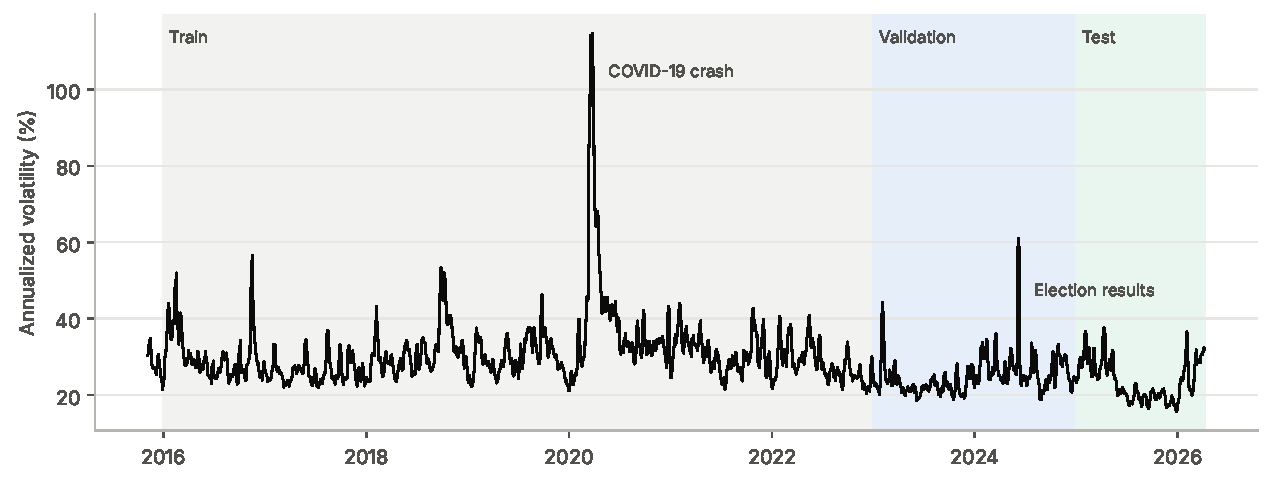
\includegraphics[width=\textwidth]{fig_rv_timeline.pdf}
\caption{Average annualized intraday volatility across the 95 stocks (5-day average) with the three
sample periods.}
\label{fig:timeline}
\end{figure}

The test period is calmer than training on average (Figure~\ref{fig:timeline}), but it includes the
tariff shock of April 2025 and the rise in volatility in early 2026.

\section{Methodology}

\subsection{Econometric benchmarks}

\textbf{HAR-RV} \citep{corsi2009}, estimated by OLS separately for each stock:
\begin{equation}
RV_{t+1}=\beta_0+\beta_D RV_t+\beta_W RV^{(5)}_t+\beta_M RV^{(22)}_t+\varepsilon_{t+1},
\end{equation}
where $RV^{(5)}_t$ and $RV^{(22)}_t$ are 5- and 22-day averages. \textbf{log-HAR} is the same
regression in logs, with forecast $\exp(\hat y+s^2/2)$ to correct for the log-normal bias. Validation
forecasts use coefficients from 2016--2022; test forecasts re-estimate on 2016--2024.

\textbf{EGARCH(1,1)-t} \citep{nelson1991} for daily returns,
\begin{equation}
\log\sigma_t^2=\omega+\beta\log\sigma_{t-1}^2+\alpha\left(|z_{t-1}|-E|z_{t-1}|\right)+\gamma z_{t-1},
\end{equation}
with Student-$t$ errors. Parameters are estimated on 2016--2022 only and then held fixed while the
model runs forward, so every feature on day $t$ uses returns up to $t$ and parameters that never saw
the evaluation years. The leverage term $\gamma$ is negative for 92\% of stocks (mean $-0.042$),
and persistence $\beta$ averages 0.92 (Annex Table~\ref{tab:egarch}).

\subsection{LSTM models}

All three networks share one architecture and training rule; only the inputs differ
(Table~\ref{tab:lstm}). A single network is trained on all 95 stocks. Each input is the last 22
trading days of features for one stock; a learned 8-dimensional stock embedding lets the network
adjust to each stock's volatility level. The output is $\exp(z+c)$, which is always positive, with
$c$ the mean training log RV. Inputs are logged where relevant and standardized with training-period
means. The loss is QLIKE. Each model is trained with three random seeds and the reported forecast is
the average of the three.

\begin{table}[htbp]
\centering
\caption{LSTM inputs and training settings}
\label{tab:lstm}
\small
\begin{tabularx}{\textwidth}{lX}
\toprule
Model & Inputs for each of the last 22 days \\
\midrule
HAR-RV-LSTM & $\log RV_t$, $\log RV^{(5)}_t$, $\log RV^{(22)}_t$ \\
EGARCH-LSTM & $\log \hat\sigma_t$ (EGARCH volatility), $z_t$ (EGARCH standardized shock) \\
HAR-EGARCH-LSTM & all five (ablation) \\
\midrule
Network & 2-layer LSTM (64 units, dropout 0.2) $\rightarrow$ [last hidden state, stock embedding (8)] $\rightarrow$ 64 $\rightarrow$ 32 $\rightarrow$ 1 \\
Training & Adam, learning rate $10^{-3}$ halved on plateau, weight decay $10^{-4}$, batch 256, gradient clipping 1.0, early stopping on validation QLIKE (patience 8, max 60 epochs) \\
Seeds & 11, 22, 33; forecast = average of the three networks \\
\bottomrule
\end{tabularx}
\end{table}

HAR-RV-LSTM sees exactly the information HAR uses, so any gain comes from the non-linear,
sequence-based and pooled form of the model rather than from new data. EGARCH-LSTM sees only
daily-return information. The networks are trained once and not re-trained on validation data,
whereas the HAR benchmarks are re-estimated on 2016--2024 before the test; this favours HAR.

\subsection{Evaluation}

For forecast $h$ and realized variance $RV$:
\begin{equation}
\text{MSE}=(RV-h)^2,\qquad \text{MAE}=|RV-h|,\qquad \text{QLIKE}=\frac{RV}{h}-\log\frac{RV}{h}-1 .
\end{equation}
QLIKE is the main loss \citep{patton2011}. Losses are computed on the same 29,774 test stock-days for
every model. Significance uses a panel Diebold--Mariano test \citep{diebold1995}: the loss
difference is averaged across stocks each day, and the mean of that daily series is tested with
Newey--West (5 lags) standard errors; $p$-values are Holm-adjusted within each loss. A moving-block
bootstrap (5-day blocks, 2,000 draws) gives a second confidence interval. Calibration is checked with
Mincer--Zarnowitz regressions in logs, with standard errors clustered by date.
